\question %2
\emph{Démontrez que, sous certaines hypothèses raisonnables, 
il est possible de garantir que votre modèle linéaire continu admette toujours
une solution entière, c'est-à-dire ne comportant que des quantités produites
entières chaque semaine. 
L'une de ces hypothèses est l'intégralité de la demande chaque semaine ; 
quelles sont les autres ?}

Il est possible de garantir que notre modèle linéaire continu
admette toujours une solution entière sous certaines hypothèses.
Une première hypothèse est que tous les éléments du 
vecteur \texttt{demande} soient entiers.
Il faut également que les constantes \texttt{stock\_initial}, \texttt{nb\_max\_sous\_traitant} et 
\texttt{nb\_ouvriers} soient entières bien sûr, sinon cela n'aurait d'ailleurs pas de sens physique.
Mais il est également nécessaire que \texttt{nb\_max\_heure\_sup} et $1/d_{a,h}$ soient entiers.
Notons enfin que nous supposons ces constantes positives, sans quoi notre modèle produirait des résultats aberrants,
voire pas de résultat du tout.

\subsubsection*{Preuve}
Pour le prouver, nous allons reformuler notre problème sous la forme d'un problème de flot de coût minimum.
Soit le graphe orienté $G(V,E)$, 
où $V$ représente l'ensemble des noeuds et $E$ l'ensemble des arêtes.
Il est utile à ce stade de s'aider d'un schéma représentant le graphe. 
Celui-ci est repris à la figure~\ref{fig:schemaFlot}.
$V$ compte un noeud pour chaque semaine et un noeud initial.
On a donc $V := {0, 1, 2, ..., T}$
où $0$ est le noeud initial et $s$ est le noeud de la semaine $s$.
Définissons maintenant les arêtes de notre graphe.
Pour le noeud $0$, on définit\footnote{Notations : $V^{-}(s)$ désigne l'ensemble des noeuds dont l'arête ``rentre'' dans le noeud s, à l'inverse $V^{+}(s)$ désigne les ``sortants''.}

\begin{figure}[h]
	\centering
		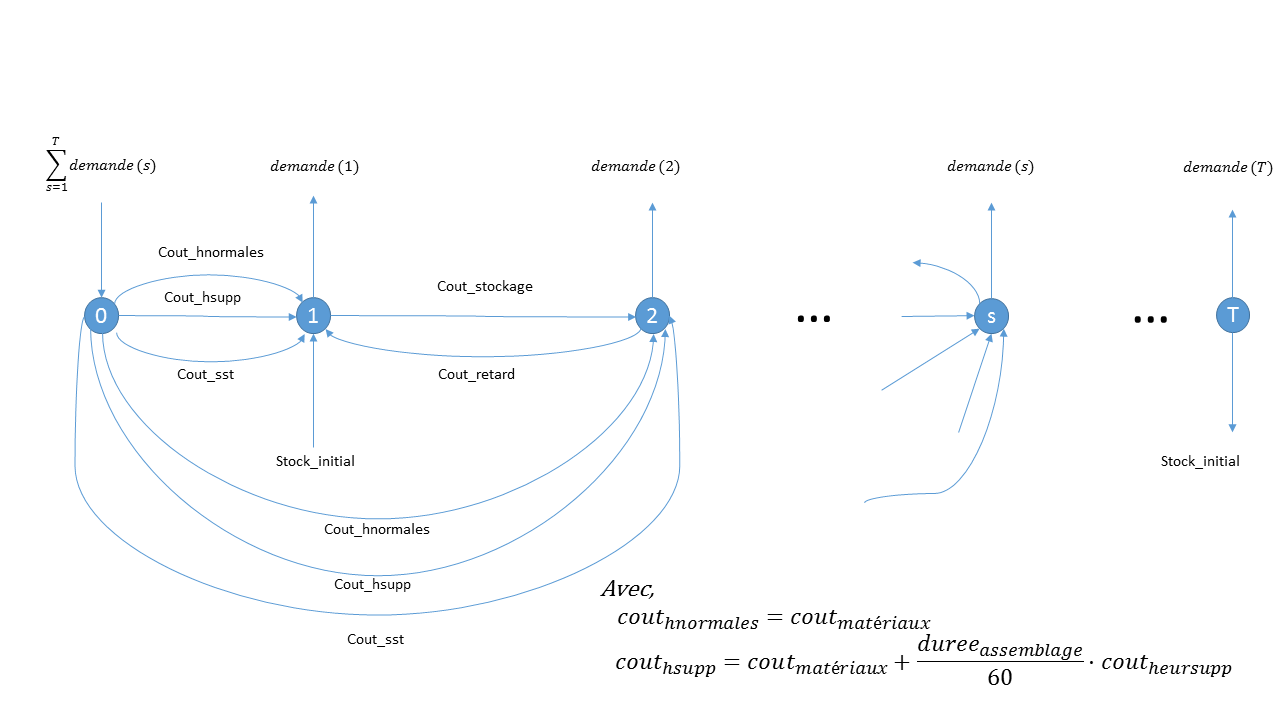
\includegraphics[scale = 0.45]{img/Schema_flot.png}
	\caption{Schéma représentant le graphe utilisé pour définir 
  le problème de flot de coût minimal.}
	\label{fig:schemaFlot}
\end{figure}

\[ V^{+}(0) = \{s_1, s_2, s_3 \quad \forall s \ne 0\} \]
avec
\[ \{(0, s_1), (0, s_2), (0, s_3)\} \in E \quad \forall s. \]
$s_1$, $s_2$, $s_3$ représentent les différentes manières de produire les smartphones, c'est-à-dire les ouvriers au salaire normal, les ouvriers au salaire des heures supplémentaires et la sous-traitance.
Il y a donc trois arcs entre les noeuds $0$ et $s$.
Pour le noeud initial,
\[ V^{-}(0) = \emptyset \]
Définissons ensuite les arêtes des noeuds correspondants aux semaines
\[ V^{+}(s) = \{s+1\} \qquad \forall s \ne 0 \]
avec 
\[ \{(s, s+1)\} \in E \qquad \forall s \ne 0, T \]
Et,
\[ V^{-}(s) = \{0, s-1\} \qquad \forall s \ne 0 \]
avec
\[ \{(s-1, s)\} \in E \qquad \forall s \ne 0, 1 \]
Nous devons encore définir les termes sources pour chaque noeud ainsi que les capacités maximales pour chaque arc.
Soit
\[ b_s = - \texttts{demande}(s) \qquad s \in V \backslash \{0\} \]
Et 
\[ b_0 = \sum_{s=1}^{T} \texttts{demande}(s) \]  
On a aussi
\[ b_1 = \texttts{stock\_initial} \]
Et
\[ b_T = - \texttts{stock\_initial} \]
Soient $h_{ij}$ avec $(i, j) \in E$ les capacités maximales dans l'arc $(i, j)$.
On a $\, \forall s \ne 0$ 
\begin{align*}
  h_{0, s_1} &= 35\cdot \texttts{nb\_ouvriers}/ d_{a,h} \\
  h_{0, s_2} &= \texttts{nb\_max\_heure\_sup}\cdot\texttts{nb\_ouvriers}/ d_{a,h} \\
  h_{0, s_3} &= \texttts{nb\_max\_sous\_traitant} 
\end{align*}
Le graphe maintenant défini, 
on peut définir le problème de minimisation suivant :
\paragraph{Variables}
Soit $x_{ij}$ le flot dans l'arc $(i, j)$.
\paragraph{Objectif}
Le coût total est minimisé.
\[ \sum_{(i, j) \in E} c_{ij} x_{ij} \]
\paragraph{Equations} Le flot est conservé en chaque noeud
\[ \sum_{k \in V^{+}(i)} x_{ik} - \sum_{k \in V^{-}(i)} x_{ki} 
  = b_i \qquad i \in V
\]
Les capacités maximales ne sont pas dépassées
\[ 0 \leq x_{ij} \leq h_{ij} \qquad (i, j) \in E \]

On peut maintenant utiliser le théorème suivant pour conclure que, si nos hypothèses sont vérifiées, notre problème admettra au moins une solution entière.
\paragraph{Théorème}
Si les demandes $b_i$ et les capcités $h_{ij}$ d'un problème de flot de coût minimum sont entières alors il existe une solution optimale entière.\footnote{En regardant de plus près la démonstration de ce résultat, on note également que chaque sommet est entier. Cependant, ce théorème ne nous dit \emph{pas} que \emph{toutes} les solutions optimales sont entières.}